% paper/sections/casestudy1.tex — Case Study 1: Phoneme (smoothing, FPCA, classification)
% Every number below is a macro written by paper/code/casestudy1.py into
% sections/cs1_numbers.tex (drift gate: paper/code/check_cs_numbers.py).
% Auto-generated by paper/code/casestudy1.py -- do not edit.
% Regenerate: PYTHONPATH=scripts:paper/code python paper/code/casestudy1.py
% Drift gate: PYTHONPATH=scripts:paper/code python paper/code/check_cs_numbers.py
\newcommand{\csOneNCurves}{400}
\newcommand{\csOneNPerClass}{80}
\newcommand{\csOneNClasses}{5}
\newcommand{\csOneNFull}{4{,}509}
\newcommand{\csOneNPoints}{256}
\newcommand{\csOneSmoothNBasis}{15}
\newcommand{\csOneSmoothN}{20}
\newcommand{\csOneRawShown}{3}
\newcommand{\csOneNComp}{4}
\newcommand{\csOneVarPCOne}{55.6}
\newcommand{\csOneVarPCTwo}{18.4}
\newcommand{\csOneVarPCThree}{4.4}
\newcommand{\csOneVarPCFour}{1.9}
\newcommand{\csOneCumVarThree}{78.4}
\newcommand{\csOneCumVarFour}{80.3}
\newcommand{\csOneCVAcc}{88.3}
\newcommand{\csOneCVFolds}{0.900, 0.875, 0.813, 0.938, 0.888}
\newcommand{\csOneCVAccFPCLDA}{88.3}
\newcommand{\csOneRecallAa}{58}
\newcommand{\csOneRecallAo}{53}
\newcommand{\csOneRecallDcl}{77}
\newcommand{\csOneRecallIy}{67}
\newcommand{\csOneRecallSh}{79}
\newcommand{\csOneAaAoConfused}{42}
\newcommand{\csOneAaAoTotal}{160}


\subsection{Smoothing, FPCA, and Classification: Phoneme Data}
\label{subsec:cs1-phoneme}

We use a balanced, seeded subset of the phoneme log-periodogram data of
\citet{hastie_buja_tibshirani_1995}: \csOneNCurves{} of the \csOneNFull{} curves
in the file distributed with \emph{The Elements of Statistical Learning},
\csOneNPerClass{} from each of \csOneNClasses{} phoneme classes (\textit{aa},
\textit{ao}, \textit{dcl}, \textit{iy}, \textit{sh}; drawn with \texttt{numpy}
seed~0), each recorded at \csOneNPoints{} frequency points.  (A related version
of these data is analysed by \citet{ferraty_vieu_2006}.)  Results on this
subset are therefore not directly comparable with published results on the
full data.  Each curve is a digitised acoustic spectrum, and the
classification task is to recover the phoneme class from its spectral shape.
This study demonstrates three core \texttt{fdars} capabilities in sequence:
penalised smoothing, functional principal component analysis (FPCA), and
cross-validated classification.

\paragraph{Smoothing.}
Raw log-periodogram curves carry measurement noise.  We apply roughness-penalised
B-spline smoothing (\texttt{fdars.basis.smooth\_basis\_gcv}) with
\csOneSmoothNBasis{} basis functions to a representative subset of
\csOneSmoothN{} curves, selecting the penalty automatically via generalised
cross-validation \citep{craven_wahba_1979,ramsay_silverman_2005}.
Figure~\ref{fig:cs1-smooth} shows the raw spectra alongside the fitted smooth
curves for each class; the smoothed curves retain the phoneme-specific spectral
peaks while suppressing high-frequency noise.

\paragraph{FPCA.}
FPCA is performed on all \csOneNCurves{} curves via
\texttt{Fdata.to\_pc(n\_comp=\csOneNComp)} \citep{ramsay_silverman_2005}.  The
first four principal components explain
$[\csOneVarPCOne, \csOneVarPCTwo, \csOneVarPCThree, \csOneVarPCFour]\%$ of
the total (quadrature-weighted) variance: \csOneCumVarThree\% jointly for the
first three and \csOneCumVarFour\% for all four.  The scores scatter in
Figure~\ref{fig:cs1-fpca} shows that \textit{dcl}, \textit{sh} and, largely,
\textit{iy} separate clearly in the PC1--PC2 plane, whereas the acoustically
similar vowels \textit{aa} and \textit{ao} overlap substantially: a
cross-validated linear discriminant on the first two scores alone recovers
\csOneRecallDcl{}, \csOneRecallSh{} and \csOneRecallIy{} of the
\csOneNPerClass{} \textit{dcl}, \textit{sh} and \textit{iy} curves, but
confuses \textit{aa} and \textit{ao} with each other in \csOneAaAoConfused{}
of their \csOneAaAoTotal{} curves.

\paragraph{Classification.}
We evaluate a scikit-learn \texttt{Pipeline} that chains an \texttt{fdars}
\texttt{FPCATransformer} (\csOneNComp{} components) with scikit-learn's
\texttt{LinearDiscriminantAnalysis} by 5-fold stratified cross-validation, so
that FPCA is fitted once per training fold.  The pipeline achieves a mean CV
accuracy of \csOneCVAcc\% on held-out data (fold scores:
$[\csOneCVFolds]$); the one-step \texttt{fdars} classifier
\texttt{FPCLDAClassifier(ncomp=\csOneNComp)}, which performs the FPCA
internally, gives the same mean accuracy (\csOneCVAccFPCLDA\%) on the same
folds.  The remaining errors are concentrated in the \textit{aa}/\textit{ao}
pair noted above.
The analysis, including every number above, is reproduced by
\texttt{paper/code/casestudy1.py}, which also generates both figures
deterministically.

\begin{figure}[tbp]
  \centering
  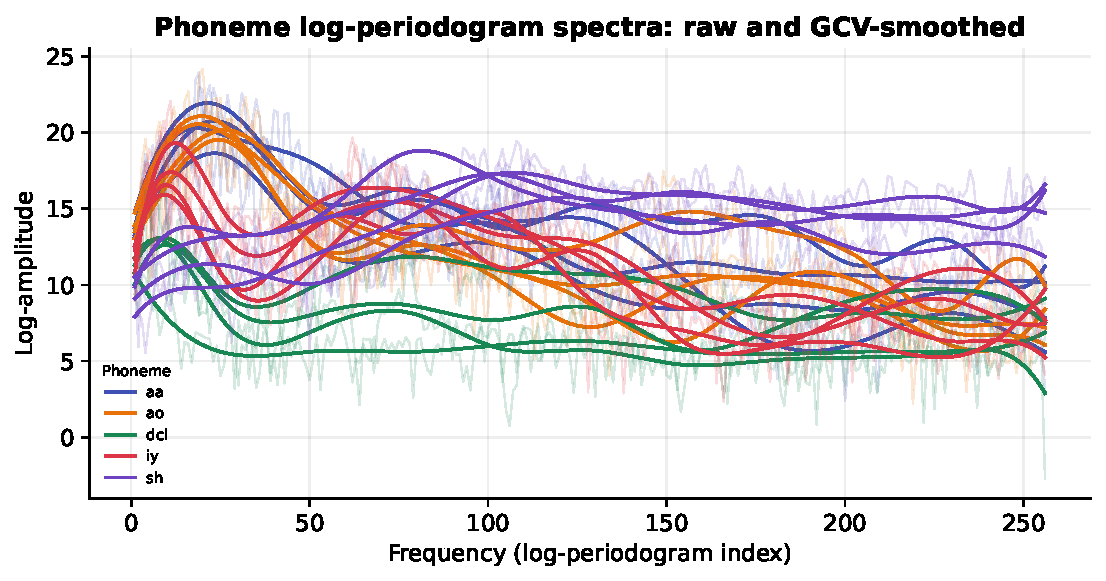
\includegraphics[width=\textwidth]{figures/cs1_phoneme_smooth.pdf}
  \caption{Phoneme log-periodogram spectra (balanced \csOneNCurves-curve subset,
    \csOneNClasses{} classes).  Light traces: raw curves (\csOneRawShown{} per
    class); bold traces: GCV B-spline smoothed curves (\csOneSmoothNBasis{}
    basis functions, penalty selected by GCV\@).  Colours identify phoneme
    classes (\textit{aa}, \textit{ao}, \textit{dcl}, \textit{iy},
    \textit{sh}).}
  \label{fig:cs1-smooth}
\end{figure}

\begin{figure}[tbp]
  \centering
  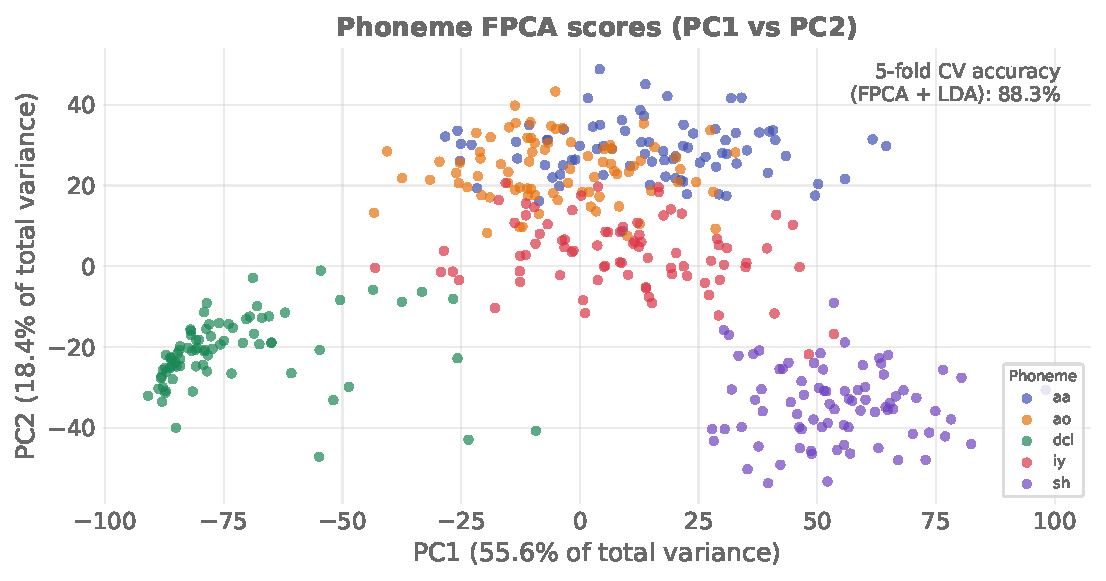
\includegraphics[width=\textwidth]{figures/cs1_phoneme_fpca.pdf}
  \caption{FPCA scores scatter for the phoneme data (PC1 vs PC2, colour-coded
    by class).  The first two principal components explain \csOneVarPCOne\% and
    \csOneVarPCTwo\% of total variance respectively; \textit{dcl},
    \textit{iy} and \textit{sh} are well separated in this projection, while
    \textit{aa} and \textit{ao} overlap.  The box reports the
    \csOneCVAcc\% 5-fold CV accuracy of \texttt{FPCATransformer} +
    \texttt{LinearDiscriminantAnalysis} on \csOneNComp{} components.}
  \label{fig:cs1-fpca}
\end{figure}
